%\documentclass{article}
%\usepackage[utf8]{inputenc}

\documentclass[12pt]{article}
\usepackage{graphicx} % This lets you include figures
\usepackage{hyperref} % This lets you make links to web locations
\graphicspath{ {./images/} }

\usepackage[rightcaption]{sidecap}
\usepackage{subcaption}
\usepackage{wrapfig}

\usepackage{float}

\usepackage{imakeidx}

\makeindex


\title{PLANTHY\\ {\large A smart care for a healthy pant}}
\author{Alejandro Vargas Pérez\\
Victor Loureiro Sancho\\
Manuel Cintero Romera\\
Alonso Espasandin Hernan\\
Giorgia Baron\\
Francesco Inchingolo
} 
\date{\today}

\begin{document}
\maketitle{}

\tableofcontents

\clearpage
\newpage

\section{Introducción al Sistema Planthy}

%\maketitle{Setup}

\subsection{Qué es Planthy?}
Planthy es un completo sistema autónomo para la seguridad de las plantas. 

\begin{figure}[H]
	\centering
	
\includegraphics[scale=1.1]{logo}
	\caption{Planthy}
	\label{fig:planthy}
\end{figure}
Aquí hay una lista de algunas características peculiares:

\begin{itemize}
 \item Control de tiempo completo y monitoreo del estado de salud para todas las plantas
 \item Esencial en ambientes insalubres
 \item Numerosas posibilidades de expansión de sensores y software según tipo de entorno
 \item Fácil de usar
 \item No hay dispositivo werarable adicional
 \item Muy asequible
\end{itemize} 



El Sistema Planthy ofrece una herramienta útil y eficiente para cuidar la salud de plantas siempreverdes de interiores.
A través del empleo de sensores de agua, humedad, temperatura y luz permite la monitorización continua del estado fisiológico de la planta en examen, proporcionando un sistema de mensajes y notificaciones que avisen al usuario sobre su bienestar. 
Lo que distingue el prototipo Planthy de otros sistemas de monitorización vegetal es que proporciona el cálculo directo y en tiempo real del Indice de Vegetación de Diferencia Normalizada (NDVI, Normalized Difference Vegetation Index): a través de la captura y procesado de la imagen de la planta por medio de una cámara de IR, el sistema aplica la función NVDI a dicha imagen de entrada y, a continuación, utiliza un mapa de color o una rampa de color para mostrar el resultado. Dependiendo del valor adquirido por el índice NDVI, el usuario podrá obtener de manera muy sencilla e inmediata informaciones sobre el posible estado patológico de la planta, garantizando cuanto antes un tratamiento precoz y preventivo.  



\subsection{Organización del manual}
El manual del usuario consta de cinco secciones: Información general, Resumen del sistema, Primeros pasos, Usando el sistema y reportando.
\\La sección de Información general explica en términos generales el sistema y el propósito para el cual se encuentra destinado.
\\La sección Resumen del sistema proporciona una descripción general del sistema. El resumen describe los usos de los requisitos de hardware y software del sistema, la configuración del sistema, los niveles de acceso de los usuarios y
El comportamiento del sistema en caso de cualquier contingencia.
La sección de introducción explica cómo obtener Planthy e instalarlo en el dispositivo. La sección
Presenta brevemente el menú del sistema.
El uso de la sección Sistema proporciona una descripción detallada de las funciones del sistema.
La sección de informes describe cómo se presenta la información recopilada por la solicitud y cómo
Para acceder a la información.

\newpage

\section{Arquitectura general del sistema}
A continuación se representa la arquitectura general del sistema que se propone, evidenciando las principales conexiones entre los sensores utilizados, la càmara, la bomba de agua y la interfaz gràfica con la que el usuario se relaciona para llevar a cabo la monitorizaciòn de la planta. Para el correcto utilizo del sistema, no se requiere un particular conocimiento previo por parte del usuario, solo es necesaria una atenta lectura de esta guìa para aprender las pautas bàsicas que permiten el empleo óptimo del protòtipo. 

\begin{figure}[H]
	\centering
	\includegraphics[scale=.2]{schema1}
	\caption{Arquitectura hardware del sistema}
	\label{fig:start}
\end{figure}

Como se observa en Figura 1, la estructura hardware està compuesta por dos tipos de sensores para extraer informaciones cuantitativas sobre luz, humedad y temperatura del aire. Dichos sensores se conectan a la plataforma Arduino que està acoplada al modulo Raspberry Pi mediante una relaciòn Master-Slave. 
La Raspberry recibe simultaneamente las imàgenes adquisidas por la càmara, extraendo periodicamente medidas del ìndice NDVI basadas en una anàlisis de los valores RGB. 
Toda la informaciòn, resultado del procesamiento efectuado por el mòdulo Raspberry, se visualiza en la pantalla tàctil, asì que el usuario pueda enterarse en todo momento de la salud de su planta.
Cada elemento mencionado,asì como las instrucciones para el uso correcto de la interfaz, seràn descritos màs en detalle en los siguientes apartados.

\clearpage
\newpage

\section{Sensores y disposidivos utilizados}
Este capítulo muestra brevemente los sensores y todos los dispositivos que el sistema Planthy utiliza y tambien muestra cómo interpretar los valores que estos sensores adquieren. Se indican los valores ideales dentro de los cuales la planta goza de buena salud.

\subsection{Arduino}

\begin{figure}[H]
	\centering
	\includegraphics[scale=.35]{arduino}
	\caption{Arduino Nano}
	\label{fig:Arduino Nano}
\end{figure}

\subsection{Raspberry Pi}

\begin{figure}[H]
	\centering
	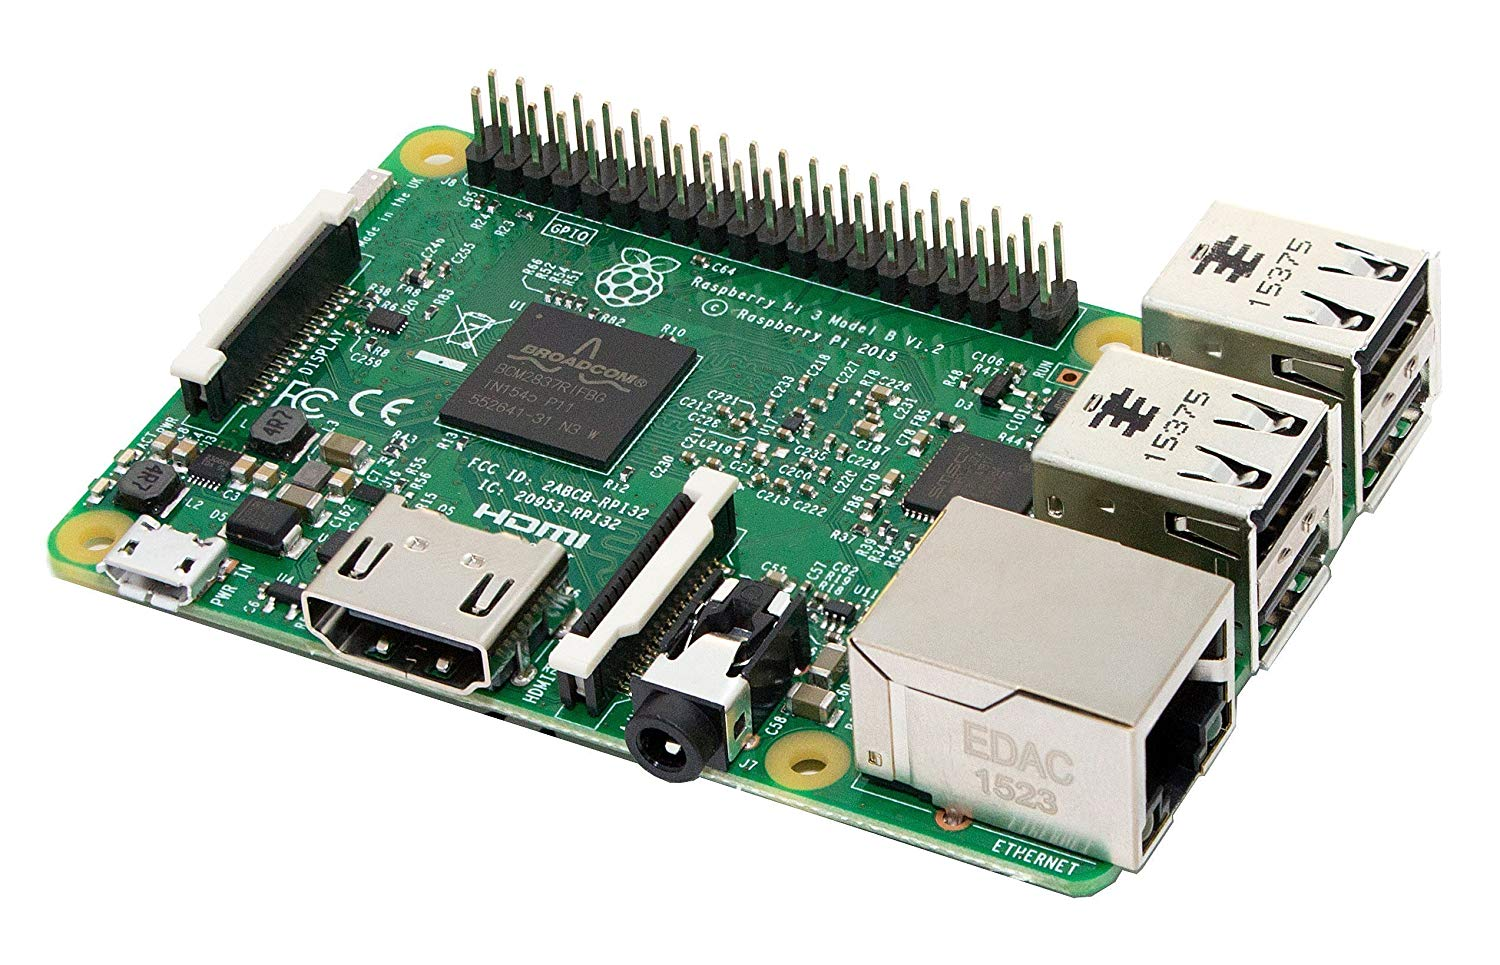
\includegraphics[scale=.16]{raspberry}
	\caption{Raspberry Pi}
	\label{fig:raspberry}
\end{figure}

\subsection{Sensor de humedad y temperatura}

\begin{figure}[H]
	\centering
	\includegraphics[scale=.12]{dht11}
	\caption{Sensor de humedad y temperatura DHT11}
	\label{fig:DHT11}
\end{figure}

\subsection{Sensor de luz}

\begin{figure}[H]
	\centering
	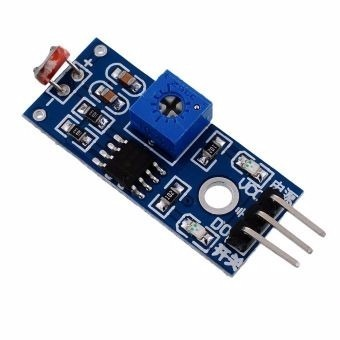
\includegraphics[scale=.45]{Luz}
	\caption{Sensor de luz TSL2591}
	\label{fig:luz}
\end{figure}

\subsection{Bomba de agua}

\begin{figure}[H]
	\centering
	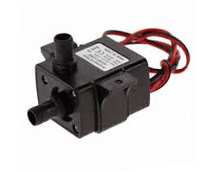
\includegraphics[scale=1.4]{arduino-bomba-agua}
	\caption{Bomba de agua}
	\label{fig:bomba}
\end{figure}

\subsection{Cámara}

\begin{figure}[H]
	\centering
	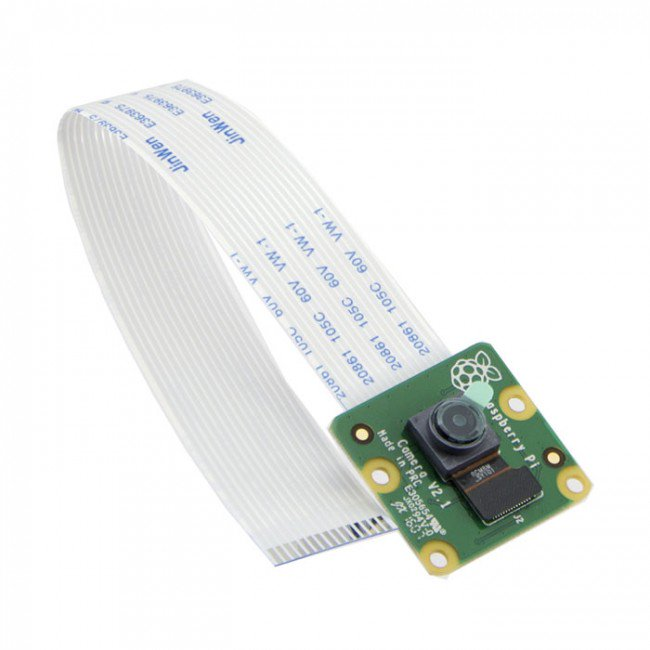
\includegraphics[scale=.25]{camera}
	\caption{Cámara PiNoir Camera V2}
	\label{fig:camera}
\end{figure}

\subsection{Pantalla}

\begin{figure}[H]
	\centering
	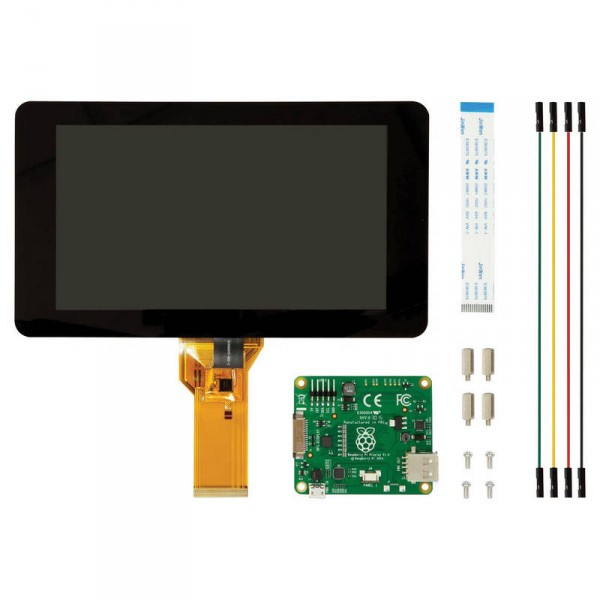
\includegraphics[scale=.5]{pantalla}
	\caption{Pantalla Táctil}
	\label{fig:pantalla}
\end{figure}

\newpage

\section{Utilizando Planthy}

\subsection{Interfaz grafica}

\begin{figure}[H]
	\centering
	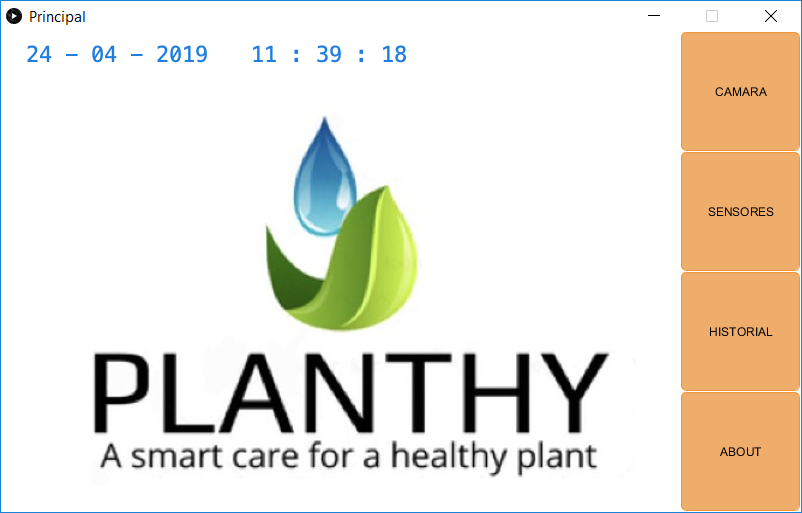
\includegraphics[scale=.6]{intro}
	\caption{Primera interfaz de la pantalla}
	\label{fig:intro}
\end{figure}

\begin{figure}[H]
	\centering
	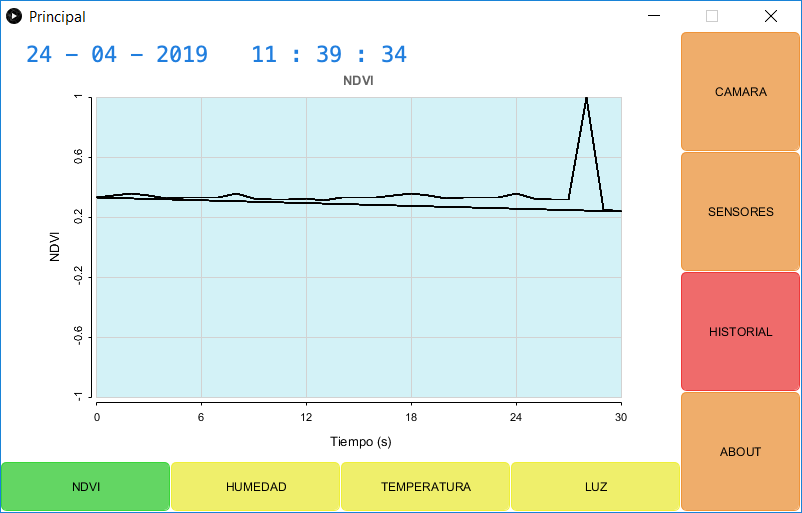
\includegraphics[scale=.6]{ndvi}
	\caption{Historial de NDVI}
	\label{fig:ndvi}
\end{figure}

\begin{figure}[H]
	\centering
	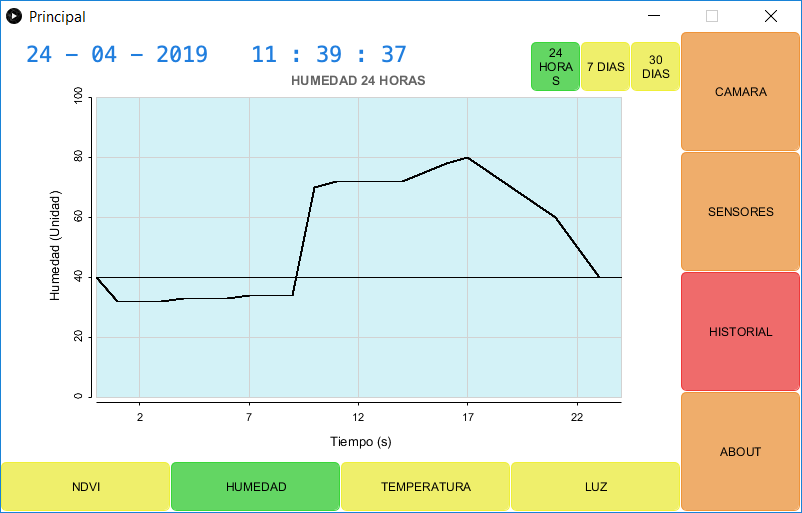
\includegraphics[scale=.6]{humed}
	\caption{Historial de la humedad}
	\label{fig:humed}
\end{figure}

\begin{figure}[H]
	\centering
	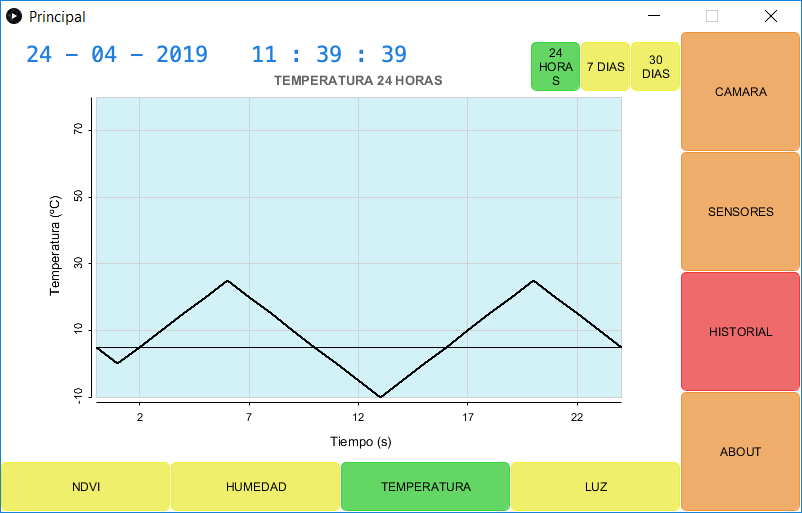
\includegraphics[scale=.6]{temp}
	\caption{Historial de la temperatura}
	\label{fig:temp}
\end{figure}

\begin{figure}[H]
	\centering
	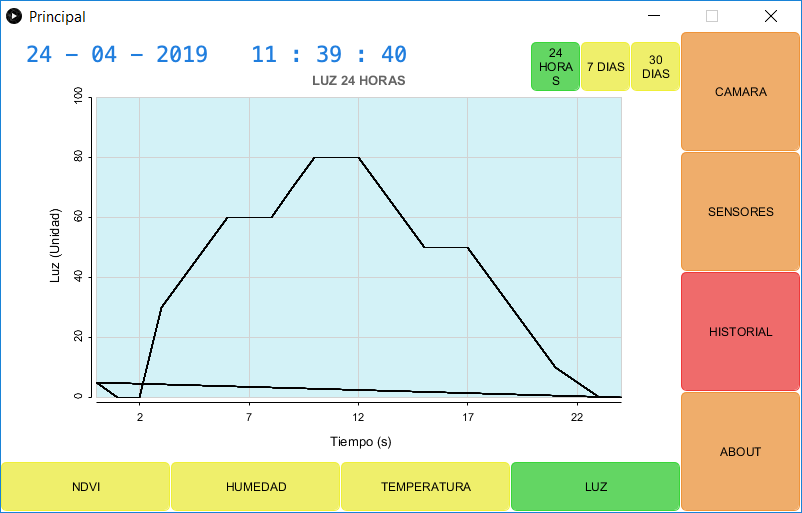
\includegraphics[scale=.6]{historial24h}
	\caption{Historial de los valore de luz}
	\label{fig:historia24h}
\end{figure}

\begin{figure}[H]
	\centering
	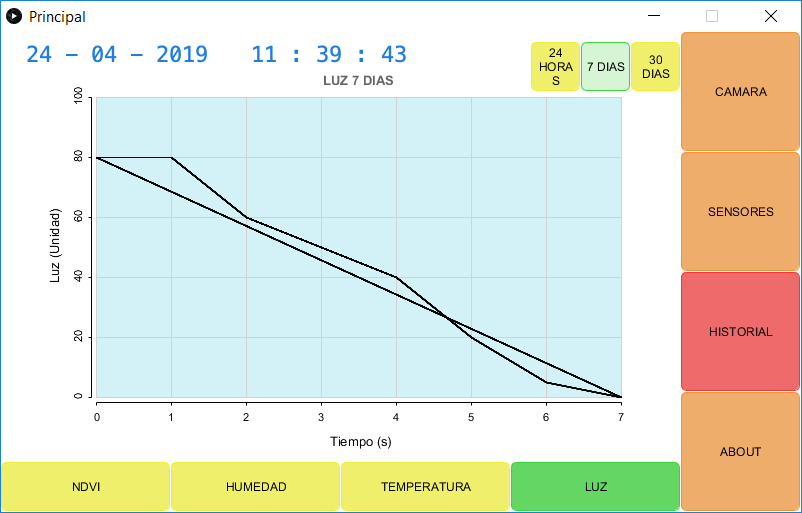
\includegraphics[scale=.6]{historial7d}
	\caption{Historial de los valore de luz en 7 dias}
	\label{fig:historial7d}
\end{figure}

\begin{figure}[H]
	\centering
	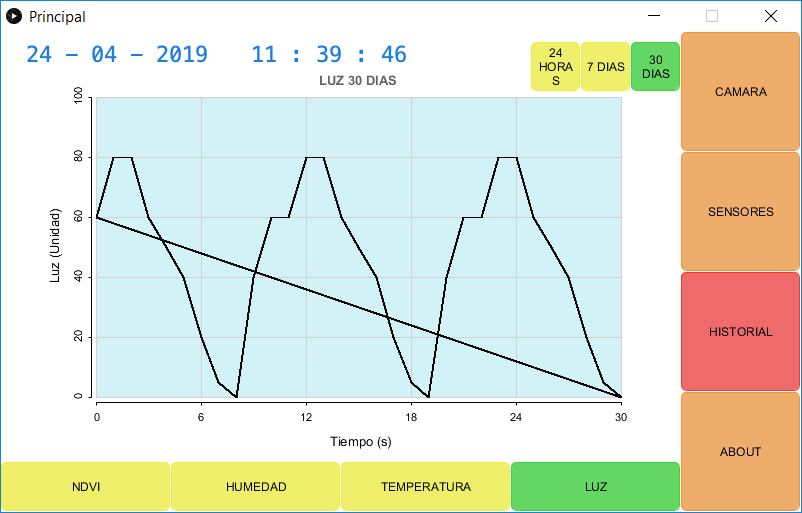
\includegraphics[scale=.6]{historial30d}
	\caption{Historial de los valore de luz en 30 dias}
	\label{fig:historia30d}
\end{figure}

\begin{figure}[H]
	\centering
	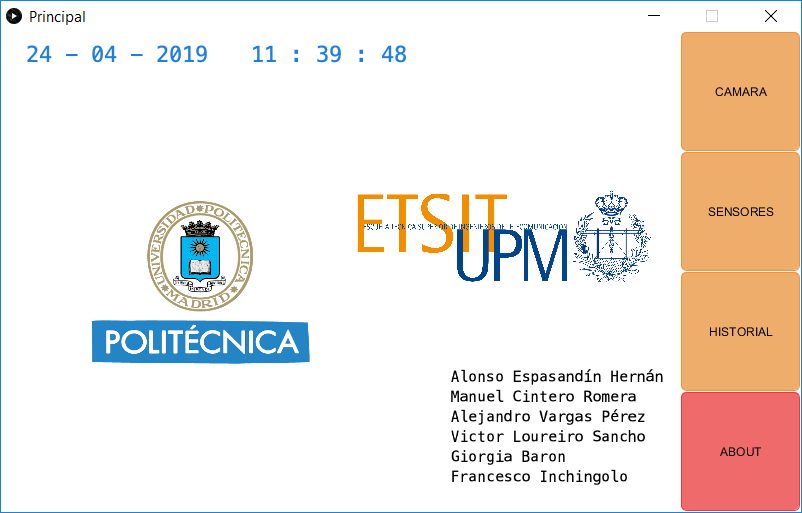
\includegraphics[scale=.6]{about}
	\caption{About us}
	\label{fig:about}
\end{figure}

\newpage

\section{Análisis de costos}


\newpage

\section{Links}

\subsection{DHT11 Temperature and Relative Humidity Sensor Module for arduino:}

\url{https://www.ebay.com/itm/New-DHT11-Temperature-and Relative-Humidity-Sensor-}
\newline
\url{https://www.amazon.es/Ferrell-Digital-Temperature Relative-Humidity/dp/B07N89PD5S/ref=sr_1_2}

\subsection{Sensor luz Fotoresistencia para Arduino:}
\url{https://www.amazon.es/SHAHIDEER-Fotoresistencia-ArduinoResistencia-fotos8}

\subsection{Módulo RGB:}
\url{https://www.amazon.es/Ils-Pieces-Colour-Module-Arduino/dp/B0769T5W25/ref=sr_1_1}

\url{https://www.ebay.com/itm/1PCS-KY-0099}

\subsection{Sensor de agua}
{https://www.digikey.es/product-detail/es/sparkfun}


\newpage

\listoffigures

\end{document}